\section{PSF Reconstruction}
	This section contains information about the models and notebooks used to reconstruc PSFs data.
	
	\subsection{Data}
	
		The data related to this project was generated using HCIpy. The main functions used for this are \filename{generate\_psf\_complex\_fields} and \filename{compute\_output\_fluxes\_from\_complex\_field} that can be found in \href{https://github.com/Dacarpe03/PLImageReconstruction/blob/main/Utils/data_utils.py}{data\_utils.py}.\\
		
		These PSFs are generated from atmospheric aberrations, NOT zernike coefficients.\\
		
		There are 90000 datapoints in this project. The paths to them are found in \href{https://github.com/Dacarpe03/PLImageReconstruction/blob/main/Utils/psf_constants.py}{psf\_constants.py}.\\
	
	\subsection{Code}
		\begin{itemize}
			\item To generate the data see the notebook \href{https://github.com/Dacarpe03/PLImageReconstruction/blob/main/PSFReconstruction/DataNotebooks/PSFGeneration.ipynb}{PSFGeneration.ipynb}.
			\item To process the data (eg. flatten, compute PSF intensities, crop PSFs) see the notebook \href{https://github.com/Dacarpe03/PLImageReconstruction/blob/main/PSFReconstruction/DataNotebooks/PSFProcessing.ipynb}{PSFProcessing.ipynb}.
			\item To train models check the folder \href{https://github.com/Dacarpe03/PLImageReconstruction/tree/main/PSFReconstruction/Training}{Training}.
			
		\end{itemize}
	\subsection{Results}
		To see all results check PART II from \filename{all.pdf}.
		
		\begin{figure*}[ht!]
			\centering
			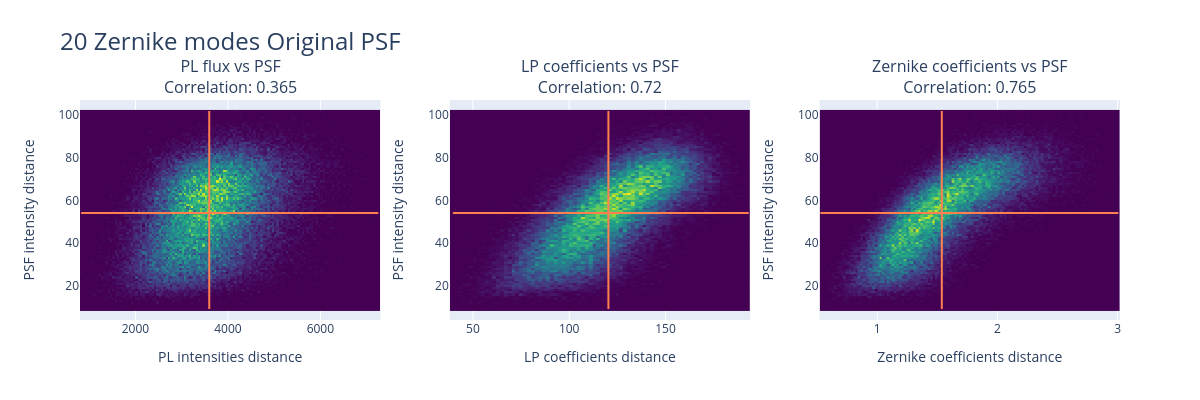
\includegraphics[width=0.9\textwidth]{pid-20mOriginalpsfdistances.png}
		\end{figure*}
		\FloatBarrier
		
		These plots are done as follows:
		\begin{enumerate}
			\item Chose a set of pairs of points. One point is a set of Zernike Coefficients, the PSF intensity they define, the LP coefficients from the overlap integral of the PSF with the LP modes and the output fluxes obtained after multiplying the transfer matrix with the LP coefficients.
			\item Compute the euclidean distances between:
				\begin{itemize}
					\item Zernike Coefficients of each point
					\item Flattened PSF intensity matrix
					\item Flattened complex LP coefficients
					\item Output flux intensities of the PSF
				\end{itemize}
			\item The coordinates of each point in the above plot represent the euclidean distance in two different optical pathway spaces. (In the first on the left the y coordinate represent the distance between a pair of points in the PSF intensities space and the x coordinate the distance between the same pair of points in the Photonic Lantern fluxes space).
		\end{enumerate}
		